%\documentclass[wcp,gray]{jmlr} % test grayscale version
\documentclass[10pt]{jmlr}% former name JMLR W\&CP
%\documentclass[pmlr]{jmlr}% new name PMLR (Proceedings of Machine Learning)

 % The following packages will be automatically loaded:
 % amsmath, amssymb, natbib, graphicx, url, algorithm2e
 \usepackage{amsmath,amssymb,graphicx,url}
 \graphicspath{ {./Figures/} }

 %\usepackage{rotating}% for sideways figures and tables
\usepackage{longtable}% for long tables

 % The booktabs package is used by this sample document
 % (it provides \toprule, \midrule and \bottomrule).
 % Remove the next line if you don't require it.
\usepackage{booktabs}
 % The siunitx package is used by this sample document
 % to align numbers in a column by their decimal point.
 % Remove the next line if you don't require it.
\usepackage[load-configurations=version-1]{siunitx} % newer version
 %\usepackage{siunitx}

% Package to make table with multi rows and columns
\usepackage{multirow}
 
 % to do
\usepackage{xcolor}
\newcommand\todo[1]{\textcolor{red}{#1}}

 % change the arguments, as appropriate, in the following:
\jmlrvolume{}
\jmlryear{}
\jmlrworkshop{STA723 -- Case Study 3}
\jmlrproceedings{}{}


\usepackage[toc,page]{appendix}


% start article
% \titlebreak
% \footnote{}
% \textsf

\title[Predictive modelling of alcohol-associated risks in college students]{Predictive modelling of alcohol-associated risks in college students}
 % Use \Name{Author Name} to specify the name.
 % If the surname contains spaces, enclose the surname
 % in braces, e.g. \Name{John {Smith Jones}} similarly
 % if the name has a "von" part, e.g \Name{Jane {de Winter}}.
 % If the first letter in the forenames is a diacritic
 % enclose the diacritic in braces, e.g. \Name{{\'E}louise Smith}

 % Authors with different addresses:
 
 \author[Binette, Morsomme]{Olivier Binette \and Raphael Morsomme}
 \date{\today} % Date, can be changed to a custom date

 % Three or more authors with the same address:
 % \author{\Name{Author Name1} \Email{an1@sample.com}\\
 %  \Name{Author Name2} \Email{an2@sample.com}\\
 %  \Name{Author Name3} \Email{an3@sample.com}\\
 %  \addr Address}

 % Authors with different addresses:
 % \author{\Name{Author Name1} \Email{abc@sample.com}\\
 % \addr Address 1
 % \AND
 % \Name{Author Name2} \Email{xyz@sample.com}\\
 % \addr Address 2
 %}

% leave editor's section empty?
%\editor{Editor's name}
% \editors{List of editors' names}

\begin{document}

\maketitle

\begin{abstract}

\end{abstract}

%%%%%%%%%%%%%%%%%%%%%%%%%%%%%%%%%%%%%%%%%%%%%%%%%%%%%%%%%%%%%
% INTRODUCTION
%%%%%%%%%%%%%%%%%%%%%%%%%%%%%%%%%%%%%%%%%%%%%%%%%%%%%%%%%%%%%
\section{Introduction}
\label{sec:intro}



The goal of our case study was to develop a predictive model of alcohol related risks in college students using information readily available to schools, in order to help (i) identify students at risk and allocate support ressources as effectively as possible; and (ii) determine other pieces of information that a school might additionally gather identify students at risk.

To address the first question, we develop a base predictive model which takes for input a student's demographic information, information about their living accomodation on or off campus, and their GPA, in order to predict a ``ressource need'' score variable. This score variable is composed of a student awareness score and three interpretable risk scores (for consumption risks, behavioural risks, and situational risks). Responses from the College Alcohol Survey were used to score individuals in these categories and train the predictive model, and the Conformal Prediction framework is used to provide prediction uncertainty quantification.

For the second question, we studied the gain in predictive performance that can be obtained using additional predictors related to student well-being and interests. These predictors are not directly related to alcohol consumption (although one of they include a survey question about the importance of partying) and could reasonably be probed for in order to help determine a student's risk. 

\subsection{Important considerations for predictive modelling}

Predictive modelling comes with particular challenges and considerations which should be addressed in the context of a real-world application. In this case study, we adress the following two points:

\begin{itemize}
\item \textbf{Meaningfulness:} We construct an interpretable and meaningful response variable disaggregated across student awareness and across three kinds of alcohol-related risks. While we do not have the subject-matter expertise necessary to properly weight the different risks, this opens up our modelling approach to scrutiny and improvement.
\item \textbf{Reliability and out of sample performance:} We provide uncertainty quantification for the predictions with exact frequentist coverage under a data representativeness assumption. In other words, we quantify the accuracy of our model through a quantity $\Delta$ such that, for any prediction $p$, $p \pm \Delta$ is a $95\%$ confidence interval for the predicted value. This $\Delta$ is obtained through the conformal prediction framework by computing the marginal distribution of the out of sample prediction error. 
\end{itemize}


Additionally, the following should be considered if a predictive model like the one we proposed were to be used in practice. We do not address these in this case study.

\begin{itemize}
\item \textbf{Fairness:} The use of age, race, gender, religion and other variables as predictors is problematic for schools under Title IX. Data quality and reliability among these groups, as well as the meaningfulness of the response variable we define for them and the practical implications of the use of such a predictive model should be carefully considered prior to any implementation.
\item \textbf{Data representativeness:} We only used data from the 2001 College Alchol Survey. The information it contains may be outdated and is certainly unrepresentative of the student population at any given school. Post-stratification and other adjustments could be carried out in applications.
\end{itemize}









\section{Methodology}

Since we do not expect the relationship between the predictors and the response to be linear, we opt for a flexible predictive model. We choose the random forest algorithm because it offers good predictive power and requires little tuning . Note that due to the size of the data set, a random forest takes 30 minutes to fit, thereby limiting the possibility of tuning the parameters and conducting a sensitivity analysis. The parameters are $n=1,500$ trees, $m=p/3$ predictors considered at each split (where $p$ is the number of predictor, standard practice for regression) and the minimum number of observation per leaf is $5$.

To answer the main question of whether or not schools should collect more data about their student that what is already readily available to them in order to identify students at risk, we fit a random forest model to each set of predictors. We then construct prediction intervals using the conformal prediction framework and compare their average width across the two models at various significance level. If the additional set of predictors does help make more accurate predictions and are therefore \textit{useful}, then the prediction intervals of the model will be tighter, that is, more informative.

\subsection{Conformal Prediction}

Conformal prediction is a framework conceptualized by Vapnik, Gammermand an Vovk in the late 90's to complement point predictions with a measure of certainty that enjoys certain properties. In the regression settings, this takes the form of prediction intervals. These prediction intervals enjoy the following properties. First, they are valid in the frequentist sense for a finite sample size, meaning that they cover the true response of the observation $\epsilon \%$, where $\epsilon$ is a set significance level, and that this property is not asymptotic. Second, the framework is distribution-free and universal. The latter qualification means that the framework can be applied to any prediction algorithm that outputs a point estimate (e.g. ridge regression, neural network, $k$-nearest neighbor algorithm, random forest, to name a few). Third, these intervals can also be individualized to each observation, that is, an observation that is easy to predict will have a tight interval while an observation that is difficult to predict will have a wider interval. Finally, using \textit{inductive} conformal prediction, the construction of the intervals is computationally cheap, only requiring fitting the predictive model once. This can be compared to the bootstrap approach to the construction of prediction intervals which requires numerous fittings of the predictive models. In our case, since the random forest takes $30$ minutes to fit, bootstrap would not have been an option. It is worth noting that the only assumption made o construct conformal prediction prediction intervals is the exchangeability of the observations.

We use the \textit{inductuve conformal framework} to construct predictive interval. The methods proceeds as follows. Given a labeled training set $\{z_i = (x_i, y_i)\}_{i=1}^n$ and an unlabeled test observation $x_{n+1}$,
\begin{enumerate}
	\item partition the training set into a \textit{proper training} set $\{z_j\}_{j=1}^l$ and a \textit{calibration} set $\{z_k \}_{k=l+1}^n$,
	\item fit the predictive model $m$ on the proper training set,
	\item compute the predictions $\hat{y}_k$ on the calibration set and the anomaly scores
	$$a(z_k, m) = |\hat{y}_k - y_k|, \quad k = l+1, \dots, n$$,
	\item identify $a_\epsilon$, the $\epsilon^{\text{th}}$ percentile of the $\{a\}_{k=l+1}^n$,
	\item compute the prediction $\hat{y}_{n+1}$ on the test observation and set the prediction interval to be
	$$\{y: |\hat{y}_{n+1} - y| < a_\epsilon\}$$.
\end{enumerate}
Note that these intervals will be the same of every observation. In order to make them individualized, one need to use a anomaly function function such that
$$a(z_k, m_1, m_0) = \dfrac{|\hat{y}_k - y_k|}{exp(\sigma_k)}$$
where $\hat{y}_k$ is the prediction of the response variable made model $m0$ and $\sigma_k$ is the prediction of the log absolute error $log(|\hat{y}_k - y_k|)$ made by a second model $m1$ trained on the calibration set. The log-exponentiation trick is used to ensure that the anomaly values $a(z_k, m_1, m_0)$ are positive.

We use the following set-up: the test set consists of $10\%$ of the data set, the calibration set consists of $30\%$ of the training set and we repeat the procedure $10$ times to obtain the expected width of prediction
intervals for each model at various significance levels.



\section{Results}
\label{sec:results}

Table 1 indicates that, given a significance level, the conformal prediction intervals are valid in the frequentist sense up to statistical fluctuations. \figureref{fig:conformal} shows the distribution of the prediction intervals. We observe that the model with the larger set of predictors produces intervals that are tighter than those of the base model. Tables 2 and 3 indicate the $10$ variables with the highest contribution to each model. Race appears to be an important predictor in both models. 

\section{Discussion}
\label{sec:conclusion}

It seems that only the student's attitude towards parties seems to be complementing the variables of the base model. In fact, among the $5$ most important variables of the augmented model, it is the only one that is not present in the base model. Interestingly, it is also the most important variable of the augmented model by a large margin, indicating that collecting this variable will help schools identify more efficiently students at risk.



\newpage
\appendix

\section{Figures}

% latex table generated in R 3.5.2 by xtable 1.8-3 package
% Mon Feb 17 15:58:32 2020
\begin{table}[ht]
\centering
\begin{tabular}{rrlrr}
  \toprule
 & Significance & Set of Predictors & Mean Width & Coverage \\ 
  \midrule
1 & 0.500 & Extensive & 1.138 & 0.503 \\ 
  2 & 0.500 & Restricted & 1.370 & 0.501 \\ 
  3 & 0.750 & Extensive & 1.807 & 0.754 \\ 
  4 & 0.750 & Restricted & 2.109 & 0.749 \\ 
  5 & 0.900 & Extensive & 2.513 & 0.909 \\ 
  6 & 0.900 & Restricted & 2.801 & 0.897 \\ 
  7 & 0.950 & Extensive & 2.896 & 0.954 \\ 
  8 & 0.950 & Restricted & 3.212 & 0.951 \\ 
   \bottomrule
\end{tabular}
\caption{Coverage and Mean Width of Prediction Intervals} 
\end{table}


\begin{figure}[htbp]
	\centering
	\caption{Median and inter-decile of the width distribution of the prediction intervals across different significance levels for the two models.}
	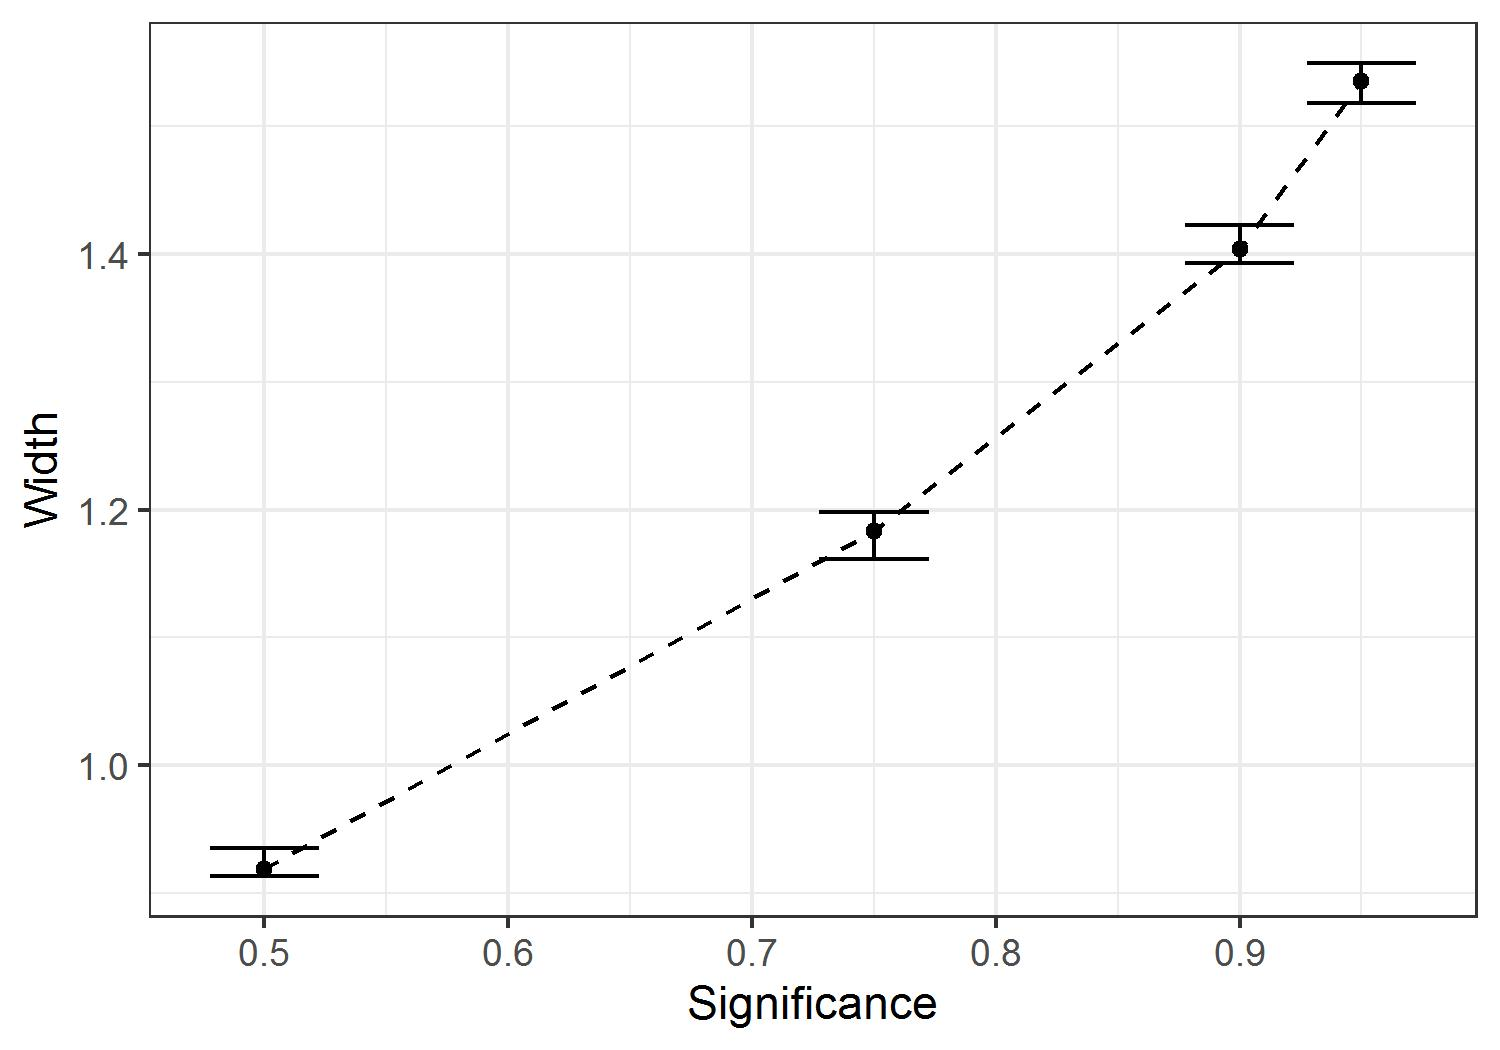
\includegraphics[width=0.9\linewidth]{conformal.jpeg}
	\label{fig:conformal}
\end{figure}

% latex table generated in R 3.5.2 by xtable 1.8-3 package
% Mon Feb 17 17:52:31 2020
\begin{table}[ht]
\centering
\begin{tabular}{rlr}
  \hline
 & Variables & Importance \\ 
  \hline
1 & race & 123.5 \\ 
  2 & roommates & 91.2 \\ 
  3 & greek\_life & 90.2 \\ 
  4 & marital\_status & 72.4 \\ 
  5 & religion & 67.6 \\ 
  6 & age & 67.1 \\ 
  7 & location & 65.1 \\ 
  8 & live\_parents & 64.9 \\ 
  9 & hispanic & 42.9 \\ 
  10 & transfer & 38.9 \\ 
   \hline
\end{tabular}
\caption{Variable importance for predictive model with restricted set of predictors} 
\end{table}


% latex table generated in R 3.5.2 by xtable 1.8-3 package
% Mon Feb 17 17:52:37 2020
\begin{table}[ht]
\centering
\begin{tabular}{rlr}
  \hline
 & Variables & Importance \\ 
  \hline
1 & parties & 268.0 \\ 
  2 & religion & 77.0 \\ 
  3 & race & 72.2 \\ 
  4 & roommates & 62.1 \\ 
  5 & greek\_life & 46.4 \\ 
  6 & marital\_status & 40.9 \\ 
  7 & socialize & 40.3 \\ 
  8 & live\_parents & 38.5 \\ 
  9 & friends & 29.3 \\ 
  10 & location & 28.1 \\ 
   \hline
\end{tabular}
\caption{Variable importance for predictive model with extensive set of predictors} 
\end{table}



\end{document}